\documentclass[english,t]{beamer}
% \documentclass[english,t,aspectratio=1610, 12pt,dvipsnames, table]{beamer}
\usepackage{beamer-JA}
\usepackage{tkz-euclide}

% \usepackage{environ}
\DeclareMathAlphabet{\mathcal}{OMS}{cmsy}{m}{n}
\SetMathAlphabet{\mathcal}{bold}{OMS}{cmsy}{b}{n} %for big-O

%\beamerdefaultoverlayspecification{<+->}

\makeatletter
\newsavebox{\measure@tikzpicture}
\NewEnviron{scaletikzpicturetowidth}[1]{%
  \def\tikz@width{#1}%
  \def\tikzscale{1}\begin{lrbox}{\measure@tikzpicture}%
  \BODY
  \end{lrbox}%
  \pgfmathparse{#1/\wd\measure@tikzpicture}%
  \edef\tikzscale{\pgfmathresult}%
  \BODY
}%
\makeatother

%%%%Chapter and Section numbers%%%%% 
\newcommand{\chNum}{}
\newcommand{\secNum}{}
\newcommand{\secTitle}{Cauchy's Rigidity Theorem}
%\date{\formatdate{29}{9}{2015}}

%%%Title page%%%%%%%%
\title[Cool Math Meeting]{Art Gallery Problem}
% \day=21
% \month=8
% \year=2019 %remove to auto set date
\subtitle{}
\author{Jim Ashe}
%%change for windows/linux. note the forward slashes for windows!%%%
\titlegraphic{
\includegraphics[height=2.25cm]{pics_shared/WGU_logo.png}}
%%\titlegraphic{
\includegraphics[height=2.25cm]{/home/jim/Copy/schools/WGU/images/WGU_logo.png}}
\institute{IT College \\Computer Science}
%%%%%%%%%%%%%%%
\setbeamertemplate{caption}{\raggedright\insertcaption\par} %%removes label from figure captions
\tikzset{c/.style={every coordinate/.try,draw=#1!50!white}} %set for coord shift hack
\begin{document}
\makebeamertitle 
%%%%%%%%%%%%%%%

%%%%%
\begin{frame}{Back story}
    \begin{figure}
        \centering
        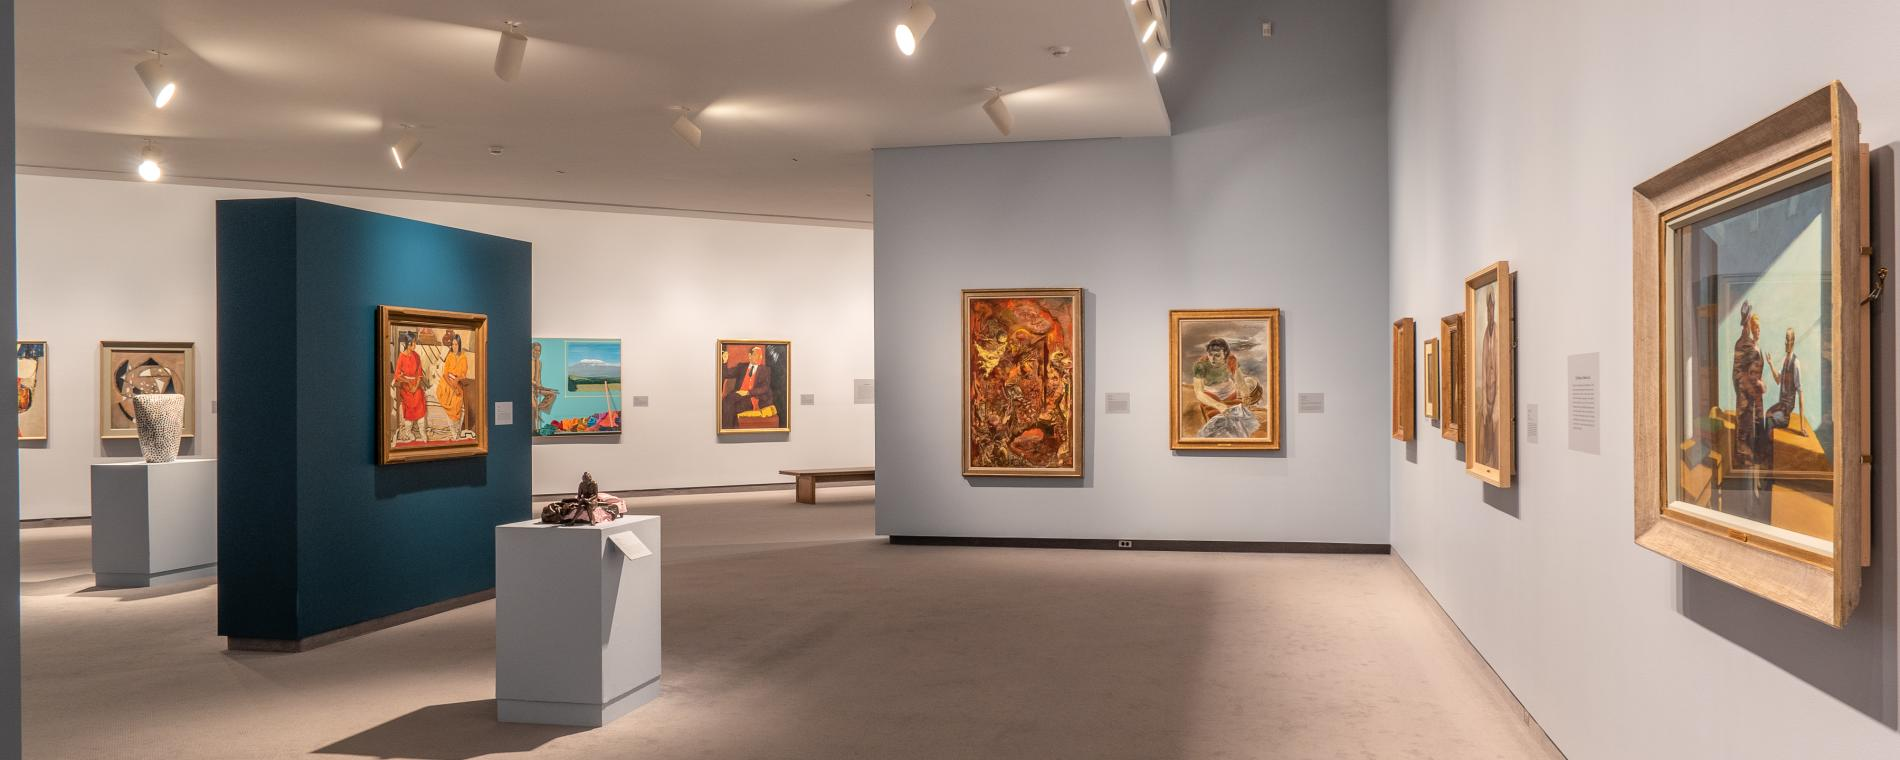
\includegraphics[width=\textwidth]{images/Visit_Wichita_Kansas_Wichita_Art_Museum_ab2f81d5-0500-4ccd-af3a-20835143dc89.jpg}
    \end{figure}
\end{frame}

%%%%%
\begin{frame}{How many guards to guard the gallery? Easy case} \label{slide-backstory}
    \def\scalePoly{2}
    \begin{center}
        \only<1>{%
            \begin{tikzpicture}[scale=\scalePoly]
                % create the node
                \node[ultra thick,draw,minimum size=6cm,regular polygon,regular polygon sides=10] (a) {};
                % draw a black dot in each vertex
                \foreach \x in {1,2,...,10}
                  \fill (a.corner \x) circle[radius=2pt];
                
                % \foreach \x in {2,...,10}
                %   \draw[dashed,<-,red,thick] (a.corner \x) to (a.corner 1);
            
                % \draw[fill=red] (a.corner 1) circle(.05cm) ;
            \end{tikzpicture}%
        }%
        \only<2>{%
            \begin{tikzpicture}[scale=\scalePoly]
                % create the node
                \node[ultra thick,draw,minimum size=6cm,regular polygon,regular polygon sides=10] (a) {};
                % draw a black dot in each vertex
                \foreach \x in {1,2,...,10}
                  \fill (a.corner \x) circle[radius=2pt];
                
                % \foreach \x in {2,...,10}
                %   \draw[dashed,<-,red,thick] (a.corner \x) to (a.corner 1);
            
                \draw[fill=red] (a.corner 1) circle(.05cm) ;
            \end{tikzpicture}%
        }%
        \only<3>{%
            \begin{tikzpicture}[scale=\scalePoly]
                % create the node
                \node[ultra thick,draw,minimum size=6cm,regular polygon,regular polygon sides=10] (a) {};
                % draw a black dot in each vertex
                \foreach \x in {1,2,...,10}
                  \fill (a.corner \x) circle[radius=2pt];
                
                \foreach \x in {2,...,10}
                  \draw[dashed,<-,red,thick] (a.corner \x) to (a.corner 1);
            
                \draw[fill=red] (a.corner 1) circle(.05cm) ;
            \end{tikzpicture}%
        }%
    \end{center}
% No time for that\dots
\end{frame}

%%%%%%%%%%%%%%%
\begin{frame}{How many guards to guard the gallery? fun case} \label{slide-problem}
    \def\scaleGraph{.65}
	\def\nodeA{\node[node_styleG] (A) at (-3,4.5) {}}
    % \def\nodeAgreen{\node[node_style, fill = green!50] (A) at (-4,0) {A}}
    \def\nodeB{\node[node_styleB] (B) at (-1.5,2.5) {}}
    \def\nodeC{\node[node_styleG] (C) at (-4.5,1) {}}
    \def\nodeD{\node[node_styleR] (D) at (-2,-4.5) {}}
    % \def\nodeDred{\node[node_style, fill = red!50] (D) at (4,-1) {D}}
    \def\nodeE{\node[node_styleG] (E) at (4.5,-3) {}}
    % \def\nodeEred{\node[node_style, fill =red!50] (E) at (3,3) {E}}
    \def\nodeF{\node[node_styleB] (F) at (4,2) {}}
    \def\nodeG{\node[node_styleR] (G) at (1.5,1) {}}
    \def\nodeH{\node[node_styleB] (H) at (-1.5,-3) {}}
    \def\nodeI{\node[node_styleR] (I) at (-1.5,1) {}}
    \def\nodeJ{\node[node_styleG] (J) at (0.425,0.5) {}}
    \def\nodeK{\node[node_styleR] (K) at (0.5,3.5) {}}
    %%%%
    \def\nodeAa{\node[node_style_blank] (Aa) at (-3,4.5) {}}
    \def\nodeBb{\node[node_style_blank] (Bb) at (-1.5,2.5) {b}}
    \def\nodeCc{\node[node_style_blank] (Cc) at (-4.5,1) {c}}
    \def\nodeDd{\node[node_style_blank] (Dd) at (-2,-4.5) {d}}
    \def\nodeEe{\node[node_style_blank] (Ee) at (4.5,-3) {e}}
    \def\nodeFf{\node[node_style_blank] (Ff) at (4,2) {f}}
    \def\nodeGg{\node[node_style_blank] (Gg) at (1.5,1) {g}}
    \def\nodeHh{\node[node_style_blank] (Hh) at (-1.5,-3) {h}}
    \def\nodeIi{\node[node_style_blank] (Ii) at (-1.5,1) {i}}
    \def\nodeJj{\node[node_style_blank] (Jj) at (0.425,0.5) {j}}
    \def\nodeKk{\node[node_style_blank] (Kk) at (0.5,3.5) {k}}


    \begin{center}
    
    \only<1>{%
        \begin{tikzpicture}[scale=\scaleGraph,shorten >=0pt, auto, node distance=3cm, ultra thick,
       node_styleG/.style={circle, draw=black,fill=black,font=\sffamily\scriptsize\bfseries},
       node_styleB/.style={circle, draw=black,fill=black,font=\sffamily\scriptsize\bfseries},
       node_styleR/.style={circle, draw=black,fill=black,font=\sffamily\scriptsize\bfseries},
       edge_style/.style={draw=black, ultra thick},label_style/.style={fill=white,text opacity =.5, anchor=center, pos=0.5}] 
            \nodeA;
            \nodeB;
            \nodeC;
            \nodeD;
            \nodeE;
            \nodeF;
            \nodeG;
            \nodeH;
            \nodeI;
            \nodeJ;
            \nodeK;
            \draw[ultra thick,black] (A) -- (B) -- (C) -- (D) -- (E) -- (F) -- (G) -- (H) -- (I) -- (J) -- (K) -- (A);
        % \draw[ultra thick, draw black] (A)-(B)
        \end{tikzpicture}%
    }%
    
    \only<2>{%
    Original proof by V.\ Chvital (1975)
    \begin{figure}
        \centering
        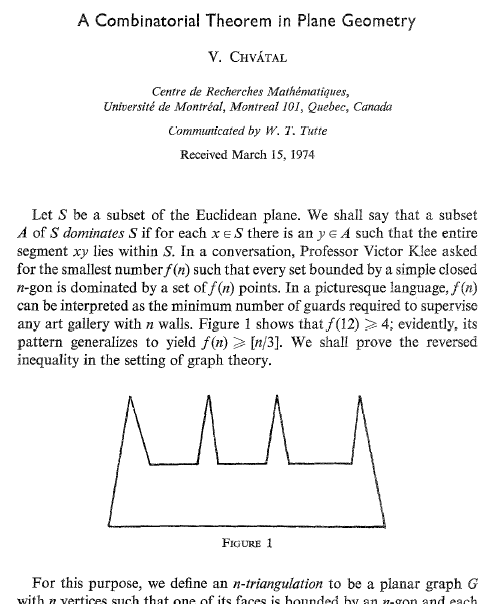
\includegraphics[width=.45\textwidth]{images/original_art_gallery_proof-1.png}
    \end{figure}
    
    }%
    
    \only<3>{%
    Original proof by V.\ Chvital (1975)
    \begin{figure}
        \centering
        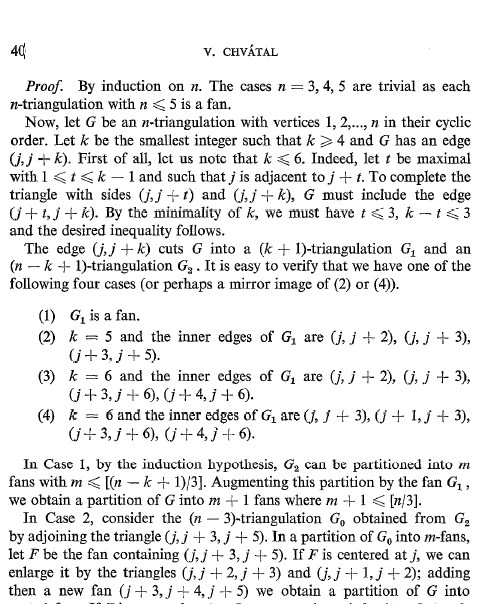
\includegraphics[width=.45\textwidth]{images/original_art_gallery_proof-2.png}
    \end{figure}
    
    }%
    
    \only<4>{%
        \begin{tikzpicture}[scale=\scaleGraph,shorten >=0pt, auto, node distance=3cm, ultra thick,
       node_styleG/.style={circle, draw=black,fill=black,font=\sffamily\scriptsize\bfseries},
       node_styleB/.style={circle, draw=black,fill=black,font=\sffamily\scriptsize\bfseries},
       node_styleR/.style={circle, draw=black,fill=black,font=\sffamily\scriptsize\bfseries},
       edge_style/.style={draw=black, ultra thick},label_style/.style={fill=white,text opacity =.5, anchor=center, pos=0.5}] 
            \nodeA;
            \nodeB;
            \nodeC;
            \nodeD;
            \nodeE;
            \nodeF;
            \nodeG;
            \nodeH;
            \nodeI;
            \nodeJ;
            \nodeK;
            \draw[ultra thick,black] (A) -- (B) -- (C) -- (D) -- (E) -- (F) -- (G) -- (H) -- (I) -- (J) -- (K) -- (A);
            \draw[thick,dashed,black] (K) -- (B);
            \draw[thick,dashed,black] (B) -- (J);
            \draw[thick,dashed,black] (I) -- (B);
            \draw[thick,dashed,black] (I) -- (C);
            \draw[thick,dashed,black] (C) -- (H);
            \draw[thick,dashed,black] (H) -- (D);
            \draw[thick,dashed,black] (H) -- (E);
            \draw[thick,dashed,black] (E) -- (G);
        % \draw[ultra thick, draw black] (A)-(B)
        \end{tikzpicture}%
    }%
    
    \only<5->{%
        \begin{tikzpicture}[scale=\scaleGraph,shorten >=0pt, auto, node distance=3cm, ultra thick,
       node_styleG/.style={circle,draw=green,fill=green!20!,font=\sffamily\scriptsize\bfseries},
       node_styleB/.style={circle,draw=blue,fill=blue!20!,font=\sffamily\scriptsize\bfseries},
       node_styleR/.style={circle,draw=red,fill=red!20!,font=\sffamily\scriptsize\bfseries},
       node_style_blank/.style={circle,draw=black,fill=black,font=\sffamily\scriptsize\bfseries},
       edge_style/.style={draw=black, ultra thick},label_style/.style={fill=white,text opacity =.5, anchor=center, pos=0.5}] 
            \nodeA;
            \nodeB;
            \nodeC;
            \nodeD;
            \nodeE;
            \nodeF;
            \nodeG;
            \nodeH;
            \nodeI;
            \nodeJ;
            \nodeK;
            
            \draw[ultra thick,black] (A) -- (B) -- (C) -- (D) -- (E) -- (F) -- (G) -- (H) -- (I) -- (J) -- (K) -- (A);
            \draw[thick,dashed,black] (K) -- (B);
            \draw[thick,dashed,black] (B) -- (J);
            \draw[thick,dashed,black] (I) -- (B);
            \draw[thick,dashed,black] (I) -- (C);
            \draw[thick,dashed,black] (C) -- (H);
            \draw[thick,dashed,black] (H) -- (D);
            \draw[thick,dashed,black] (H) -- (E);
            \draw[thick,dashed,black] (E) -- (G);
        % \draw[ultra thick, draw black] (A)-(B)
        \end{tikzpicture}%
    }%
    \uncover<6->{%
        \vspace{-1cm}
        
        \begin{equation*}
            \hspace{1cm} \text{At most }\lfloor {\frac{n}{3}} \rfloor \text{ guards.} 
        \end{equation*}
        -Fisk's short proof (1978)
    }%
    \end{center}

\end{frame}
%%%%%%%%%%%%%%%
% \begin{frame}{The back story} \label{slide-problrm}
% No time for that\dots
% \begin{columns}
%     \begin{column}{.6\textwidth}

%     \end{column}
%     \begin{column}{.4\textwidth}
%         \begin{tikzpicture}
%             \node (v1) at (-3,4.5) {};
%             \node (v10) at (0.5,3.5) {};
%             \node (v2) at (-1.5,2.5) {};
%             \node (v3) at (-4.5,1) {};
%             \node (v4) at (-2,-4.5) {};
%             \node (v5) at (4.5,-3) {};
%             \node (v6) at (4,2) {};
%             \node (v7) at (1.5,1) {};
%             \node at (-1.5,-3) {};
%             \node (v8) at (-1.5,1) {};
%             \node (v9) at (-0.5,0.5) {};
%             \draw[thick,black] (v1) -- (v2) -- (v3) -- (v4) -- (v5) -- (v6) -- (v7) -- (-1.5,-3) node (v11) {} -- (v8) -- (v9) -- (v10) -- (v1);
            
%             \draw  (v2) edge (v10);
%             \draw  (v2) edge (v8);
%             \draw  (v8) edge (v3);
%             \draw  (v3) edge (v11);
%             \draw  (v5) edge (v7);
%         \end{tikzpicture}%
%     \end{column}
% \end{columns}
% \end{frame}

% %%%%%new slide%%%%%%%
% \begin{frame}{} \label{slide-end}
%     \center
%     \Huge That is all
% \end{frame}
% %%%END SLIDES%%%
\end{document}
